\chapter{Introduction}\label{sec:intro}

When a medical professional diagnoses a patient who is seeking help for mental health-related issues, there are two 
critical factors: correctness, and timeliness of the diagnosis. The correct diagnosis 
allows the clinical psychiatrist to devise and implement the appropriate
treatment. The timeliness of the correct diagnosis means that the appropriate treatment can start as soon as possible. 
Correctly assessing the severity of a patient's psychological symptoms poses a challenge with substantial negative consequences if estimated incorrectly.
If the severity of a patient's condition
is underestimated, the patient will not receive proper treatment, and the condition
may deteriorate; if the severity of the condition is overestimated, the
patient may be unnecessarily prescribed potentially harmful medications.

Therefore, initial psychiatric evaluations of patients play a crucial role in 
both the timeliness and the correctness of the diagnosis. Such evaluations 
often contain a plethora of information, including the patient's mental health history, the family's history of mental conditions, and a detailed report of the patient's 
present symptoms. Some of this data is naturally generated in a well-structured form: e.g. as a patient's answers to a series of self-assessment survey questions.
Other parts of the evaluations come as unstructured text: doctors' notes, patients' verbatim comments, and so on.

Track 2 of the CEGS N-GRID 2016 Shared Task in Clinical Natural Language Processing
challenged the participants to 
analyze the initial psychiatric evaluations of a group of patients for the purpose of predicting the severity of their symptoms. The challenge consisted of a two-month development stage with a labeled training set and a three-day window to submit labels for an unlabeled test set. The training set was composed of real world text and survey information with redacted names and dates. 
In this paper, we describe the methods used by our team to win this challenge, by leveraging known natural language processing (NLP) and machine learning methods into a
single pipeline we called \CREATE\ (Clinical REcords Analysis Technology Ensemble) shown in Figure~\ref{fig:arch}.

\begin{figure}[h!t]
	\centering
	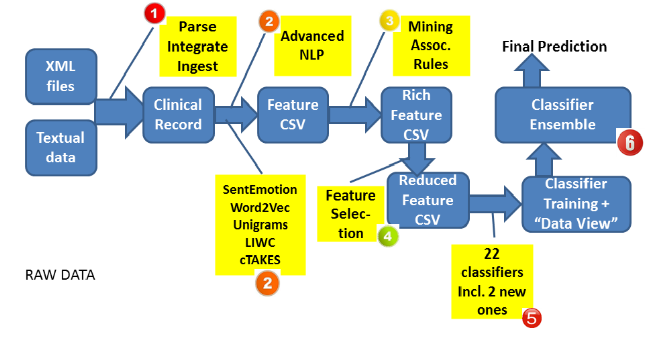
\includegraphics[width=0.95\textwidth]{figures/arch.png}
	\caption{Architecture of the \CREATE\ Framework}	
	\label{fig:arch}
\end{figure} 

The \CREATE\ framework is a machine-learning pipeline that includes several innovations. We start by taking the raw (noisy, cluttered) data provided to N-GRID challenge participants and use a data ingestion phase to ingest and clean it.
Second, we apply a host of sophisticated methods to extract a ``base'' set of  features for each clinical record from the ingested data. We expand this set of features
via a variety of methods, adding  8198 new features to the original 86. 
Third, we apply association rule mining to learn approximately 345,000 association rules
\cite{fpgrowth,c5}, and then trim them to a set of 628 predictive rules. Though association rules have been widely used in the literature for classification, we use them to generate 628 new features, one for each association rule.
Fourth, with the new total of $9284+628=9912$ features we engage a set of 
feature selection operations in order to eliminate useless features. 
Fifth, we train a total of 22 classifiers, each on seven different subsets
of features (data views). Of these, two are novel adaptations of existing Random Forest \cite{ho95,breiman01} and AdaBoost \cite{adaboost} classifiers. 
All of these classifiers build on top of the association rule classifiers developed earlier,
which is why we call them ``stackable'' in our framework. On our final step, 
we train different ensemble classifiers consisting of the subsets of best 
individual learners in order to improve the final accuracy of detection of
patient condition severity. In both the fifth and sixth steps, we do extensive k-fold cross validation and move forward from there to make our final predictions.

This is not the first time predictors have been stacked --- in the past we developed stacked regressors for predicting airline market share and demand \cite{an2016map} as well as predicting the number of hosts in a given enterprise that a malware will attack 
\cite{kang2016ensemble}.

In addition, this is not the first time our team has worked with textual medical record classification. SentEmotion is a text-based classification engine that was developed in cooperation with psychologists. Leading surveys had identified a set of signals that a victim of depression might have: for example, isolation from others. SentEmotion signals comprised some of the many features that we utilized in our final solution for the challenge \cite{coptads}.

This paper is organized as follows. In Section \ref{sec:related} we discuss prior work in this area.  Section
\ref{sec:challenge} explains the details of Track 2 of the CEGS N-GRID 2016 Shared Task in Clinical Natural Language Processing (which we, for brevity, refer to as ``the N-GRID challenge"
throughout the rest of the paper) and provides an
overview of the data we have received from the challenge organizers.  
Section~\ref{sec:overview} provides an overview of \CREATE's six-step
approach to the N-GRID challenge.  Because Step 1 (ingestion and cleaning) is 
straightforward, albeit tedious, we do not describe it.
Section~\ref{sec:features} describes the features we used, while
Section~\ref{sec:assoc-rules} describes how we selected just 628 of 345,373 association rules  generated by an off-the-shelf association rule mining engine
called FP-Growth\cite{fpgrowth}, and by adapting Quinlan's C5 decision tree
induction algorithm \cite{c45,c5} for association rule mining. 
Section~\ref{sec:selection} shows how we determined 
which features (original and extended) were irrelevant.
Section~\ref{sec:ml} describes how  we engaged in an intensive classifier training and
hyperparameter optimization procedure on seven different data views of our dataset, 
which included the  adaptations of the well-known Random Forest and AdaBoost classifiers
for our purpose.  Finally, in Section \ref{sec:ensembles} we describe how we put together 
a variety of ensembles made from the best-performing individual learners, to 
improve the final prediction accuracy.
We conclude in Section~\ref{sec:conclusion}.
